\section{S : ADTs - Queues}
\label{chap:adts_queues}

%%%%%%%%%%%%%%%%%%%%%%%%%%%%%%%%%%%%%%%%%%%%%%%%%%%%%%%%%%%%%%

\begin{frame}[fragile]
\frametitle{ADTs : Queues}
\begin{columns}[T]

\begin{column}{0.45\textwidth}
FIFO (First in, First out):
\begin{center}
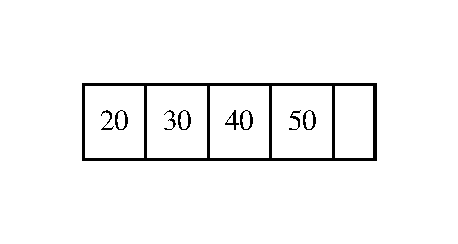
\includegraphics[scale=0.25]{../Images/Fixedq.pdf}
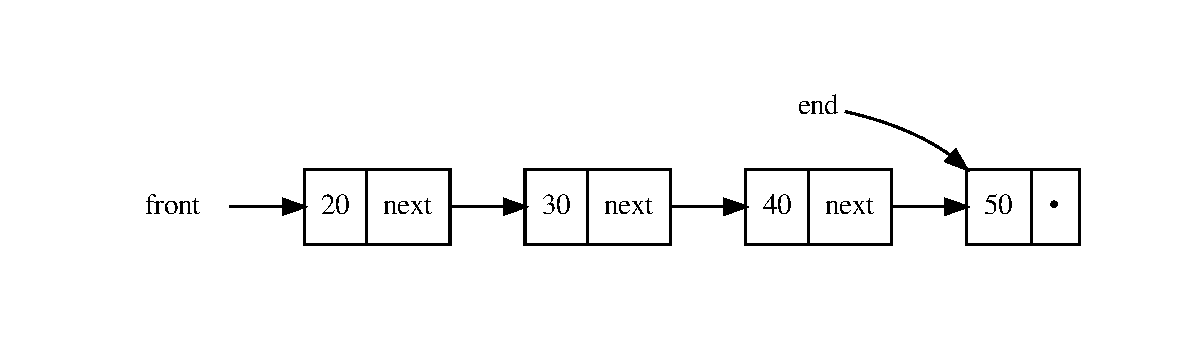
\includegraphics[scale=0.25]{../Images/Linkedq.pdf}
\end{center}
\begin{itemize}[<+->]
\item Intuitively more ``useful'' than a stack.
\item Think of implementing any kind of service (printer, web etc.)
\item Operations include \verb^enqueue^, \verb^dequeue^ and \verb^size^.
\end{itemize}
\end{column}

\pause
\begin{column}{0.45\textwidth}
\verb^queue.h^
\lstinputlisting[style=basicc,linerange={1-26}]{../../ADTs/Queue/queue.h}
\end{column}

\end{columns}
\end{frame}

%%%%%%%%%%%%%%%%%%%%%%%%%%%%%%%%%%%%%%%%%%%%%%%%%%%%%%%%%%%%%%

\begin{frame}[fragile]
\frametitle{ADTs : Queues (Fixed) I}
\begin{columns}[T]

\begin{column}{0.35\textwidth}
\verb^specific.h^
\lstinputlisting[style=basicc]{../../ADTs/Queue/Fixed/specific.h}
\end{column}

\pause
\begin{column}{0.55\textwidth}
\begin{center}
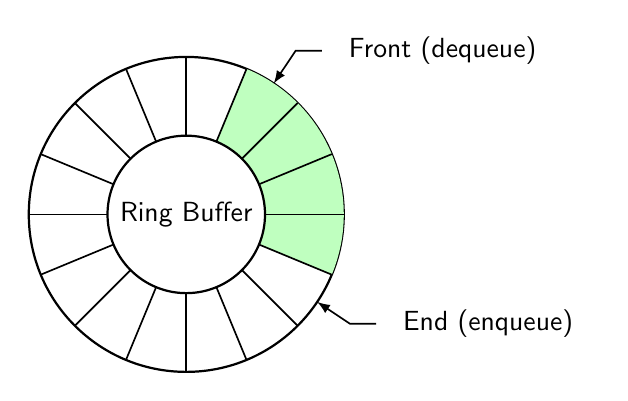
\begin{tikzpicture}[>=latex,font=\sffamily,semithick,scale=1.00]
    \draw [thick,draw=black] (0,0) circle (2);
    \fill [green!25] (0,0) -- (67.5:2) arc [end angle=-22.5, start angle=67.5, radius=2] -- cycle;
    \foreach \angle in {90,67.5,...,-67.5}
        \draw (\angle:2) -- (\angle-180:2);
    \draw [thick,fill=white,draw=black] (0,0) circle (1);
    \node [scale=1.00] at (0,0) {Ring Buffer};
    \draw [<-] (56.25:2) -- (56.25:2.50) -- +(.333,0)
        node [right,inner xsep=.333cm] (Front) {Front (dequeue)};
    \draw [<-] (-33.75:2) -- (-33.75:2.50) -- +(.333,0)
        node [right,inner xsep=.333cm] (End) {End (enqueue)};
\end{tikzpicture}
\end{center}
\end{column}

\end{columns}
\end{frame}

%%%%%%%%%%%%%%%%%%%%%%%%%%%%%%%%%%%%%%%%%%%%%%%%%%%%%%%%%%%%%%

\begin{frame}[fragile]
\frametitle{ADTs : Queues (Fixed) II}
\begin{columns}[T]

\begin{column}{0.45\textwidth}
\verb^fixed.c^
\lstinputlisting[style=basicc,linerange={1-22}]{../../ADTs/Queue/Fixed/fixed.c}
\end{column}

\pause
\begin{column}{0.45\textwidth}
\lstinputlisting[style=basicc,linerange={24-48}]{../../ADTs/Queue/Fixed/fixed.c}
\end{column}

\end{columns}
\end{frame}

%%%%%%%%%%%%%%%%%%%%%%%%%%%%%%%%%%%%%%%%%%%%%%%%%%%%%%%%%%%%%%

\begin{frame}[fragile]
\frametitle{ADTs : Queues (Fixed) III}
\begin{columns}[T]

\begin{column}{0.45\textwidth}
\lstinputlisting[style=basicc,linerange={50-70}]{../../ADTs/Queue/Fixed/fixed.c}
\end{column}

\pause
\begin{column}{0.30\textwidth}
\begin{itemize}[<+->]
\item We need a thorough testing program
\item We'll see queues again for traversing trees
\item Simulating a (slow) printer
\end{itemize}
\end{column}

\end{columns}
\end{frame}

%%%%%%%%%%%%%%%%%%%%%%%%%%%%%%%%%%%%%%%%%%%%%%%%%%%%%%%%%%%%%%

\begin{frame}[fragile]
\frametitle{ADTs : Queues (Linked) I}
\begin{columns}[T]

\begin{column}{0.45\textwidth}
\verb^specific.h^
\lstinputlisting[style=basicc,linerange={1-19}]{../../ADTs/Queue/Linked/specific.h}
\end{column}

\pause
\begin{column}{0.45\textwidth}
\verb^linked.c^
\lstinputlisting[style=basicc,linerange={1-32}]{../../ADTs/Queue/Linked/linked.c}
\end{column}

\end{columns}
\end{frame}

%%%%%%%%%%%%%%%%%%%%%%%%%%%%%%%%%%%%%%%%%%%%%%%%%%%%%%%%%%%%%%

\begin{frame}[fragile]
\frametitle{ADTs : Queues (Linked) II}
\begin{columns}[T]

\begin{column}{0.45\textwidth}
\lstinputlisting[style=basicc,linerange={34-61}]{../../ADTs/Queue/Linked/linked.c}
\end{column}

\pause
\begin{column}{0.45\textwidth}
\lstinputlisting[style=basicc,linerange={63-88}]{../../ADTs/Queue/Linked/linked.c}
\end{column}

\end{columns}
\end{frame}

%%%%%%%%%%%%%%%%%%%%%%%%%%%%%%%%%%%%%%%%%%%%%%%%%%%%%%%%%%%%%%

\begin{frame}[fragile]
\frametitle{Detour : Graphviz}
\begin{columns}[T]

\begin{column}{0.45\textwidth}
\begin{itemize}[<+->]
\item There exists a nice package, called Graphviz:
\begin{verbatim}
sudo apt install graphviz
\end{verbatim}
\item This allows the visualisation of graphs/dynamic structures
using the simple \verb^.dot^ language:
\begin{verbatim}
digraph {
   a -> b; b -> c; c -> a;
}
\end{verbatim}

\item To create a \verb^.pdf^:
\begin{verbatim}
dot -Tpdf -o graphviz.pdf examp1.dot
\end{verbatim}
\end{itemize}
\end{column}

\pause
\begin{column}{0.45\textwidth}
\begin{center}
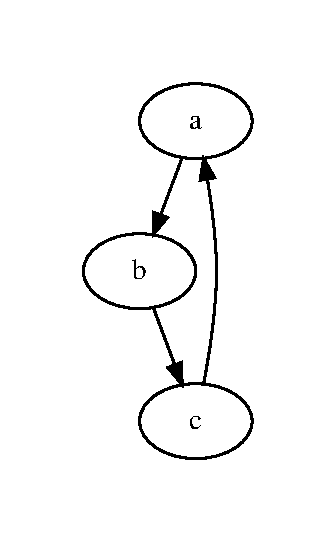
\includegraphics[scale=0.75]{../Images/graphviz.pdf}
\end{center}
\end{column}

\end{columns}
\end{frame}
